\documentclass[aspectratio=169]{beamer}
\usetheme{boxes}
\setbeamertemplate{navigation symbols}{}
\setbeamertemplate{itemize items}[circle]
\usepackage{fontspec}
\usepackage{graphics}
\usepackage{graphicx}
\usepackage{hyperref}
\usepackage{pgfplots}
\usepackage{tikz}


\setmainfont{Jost}
\setsansfont{Jost}
\setmonofont{Inconsolata}
\newfontfamily\headfamily[]{Chicago}

\newcommand{\btVFill}{\vskip0pt plus 1filll}
\newcommand{\q}[1]{\mathsf{#1}}

\tikzset{
  invisible/.style={opacity=0},
  visible on/.style={alt={#1{}{invisible}}},
  alt/.code args={<#1>#2#3}{%
    \alt<#1>{\pgfkeysalso{#2}}{\pgfkeysalso{#3}} % \pgfkeysalso doesn't change the path
  },
}

\begin{document}

\begin{frame}
  \includegraphics[width=\textwidth]{platypus-melt.jpeg}
  \btVFill
  {\Large\usebeamercolor[fg]{structure}\headfamily Predicaments with playing Platypus in parallel} \\
  \vspace{0.5em}
  Hayley Patton \hfill 26 September, 2023
  \vspace{0.5em}
\end{frame}

\tikzset{
  match/.pic={
    % Machines
    \draw (0, 0) rectangle +(3mm, 3mm);
    \draw (1cm, 0) rectangle +(3mm, 3mm);
    \draw[->] (1.5mm, 3mm) -- (7mm, 6mm);
    \draw[->] (11.5mm, 3mm) -- (11mm, 6mm);
    % Board
    \fill[yellow] (-3mm, 6mm) rectangle +(19mm, 3mm);
    \fill[green!50!black] (3mm, 6mm) rectangle +(1mm, 3mm);
    \fill[green!50!black] (-1mm, 6mm) rectangle +(1mm, 3mm);
    \fill[green!50!black] (8mm, 6mm) rectangle +(1mm, 3mm);
    \fill[green!50!black] (13mm, 6mm) rectangle +(1mm, 3mm);
    \fill[green!50!black] (13mm, 6mm) rectangle +(1mm, 3mm);
    \draw (-3mm, 6mm) rectangle +(19mm, 3mm);
  }
}

\begin{frame}
  \frametitle{Previously on \emph{Platypus Games Without Frontiers}...}
  \begin{columns}
    \begin{column}{0.5\textwidth}
      Detecting \emph{equivalent} machines reduces the number of games to run by $25\times$.

      \begin{center}
        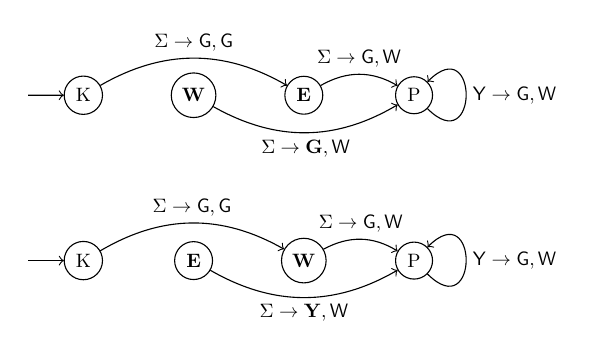
\begin{tikzpicture}[scale=0.7, every node/.style={scale=0.7}]
          \node[draw, circle] (P1) at (6, 0) {{P}};
          \node[draw, circle] (W1) at (4, 0) {{\textbf{W}}};
          \node[draw, circle] (E1) at (2, 0) {{\textbf{E}}};
          \node[draw, circle] (K1) at (0, 0) {{K}};
          \draw[->] (-1, 0) to (K1);
          \draw[->] (P1) to[in=45, out=-45, looseness=7] node[midway, right] {$\q{Y} \rightarrow \q{G}, \q{W}$} (P1);
          \draw[->] (W1) to[bend left] node[midway, above] {$\Sigma \rightarrow \q{G}, \q{W}$} (P1);
          \draw[->] (E1) to[bend right] node[midway, below] {$\Sigma \rightarrow \q{\mathbf{Y}}, \q{W}$} (P1);
          \draw[->] (K1) to[bend left] node[midway, above] {$\Sigma \rightarrow \q{G}, \q{G}$} (W1);
          
          \node[draw, circle] (P2) at (6, 3) {{P}};
          \node[draw, circle] (W2) at (2, 3) {{\textbf{W}}};
          \node[draw, circle] (E2) at (4, 3) {{\textbf{E}}};
          \node[draw, circle] (K2) at (0, 3) {{K}};
          \draw[->] (-1, 3) to (K2);
          \draw[->] (P2) to[in=45, out=-45, looseness=7] node[midway, right] {$\q{Y} \rightarrow \q{G}, \q{W}$} (P2);
          \draw[->] (W2) to[bend right] node[midway, below] {$\Sigma \rightarrow \q{\mathbf{G}}, \q{W}$} (P2);
          \draw[->] (E2) to[bend left] node[midway, above] {$\Sigma \rightarrow \q{G}, \q{W}$} (P2);
          \draw[->] (K2) to[bend left] node[midway, above] {$\Sigma \rightarrow \q{G}, \q{G}$} (E2);
        \end{tikzpicture}
      \end{center}
    \end{column}%
    \begin{column}{0.5\textwidth}
      \pause
      Multi-threading and SIMD can run 436 million games per second on a
      fast 5900X CPU.

      \begin{center}
        \begin{tikzpicture}[scale=0.7, every node/.style={scale=0.7}]
          \node at (0.75, 5.7) {Core 1};
          \draw (0, 6) rectangle (8, 4.5);
          \pic at (1.8, 4.75) {match};
          \pic at (4, 4.75) {match};
          \node at (6.75, 5.25) {$\cdots\ (8\times)$};

          \node at (0.75, 4.2) {Core 2};
          \draw (0, 4.5) rectangle (8, 3);
          \pic at (1.8, 3.25) {match};
          \pic at (4, 3.25) {match};
          \node at (6.75, 3.75) {$\cdots\ (8\times)$};

          \node at (0.75, 2.7) {Core 3};
          \draw (0, 3) rectangle (8, 1.5);
          \pic at (1.8, 1.75) {match};
          \pic at (4, 1.75) {match};
          \node at (6.75, 2.25) {$\cdots\ (8\times)$};
          
          \node at (4, 1) {$\vdots\ (24\times)$ };
        \end{tikzpicture}
      \end{center}
    \end{column}
  \end{columns}
\end{frame}

\begin{frame}
  \frametitle{GPGPU}
  One can do \emph{general-purpose} computing on a
  \emph{graphics processing unit}. A GPU has a very different
  structure to a CPU, with fewer control units controlling many
  more arithmetic units; this arrangement works well for simple,
  repetitive workloads such as:

  \begin{itemize}
  \item Physics simulations -- apply all incoming forces on each particle,
  \item Image and video editing -- apply effects to each pixel,
  \item Cryptocurrency mining -- compute many hashes in parallel,
  \item Machine learning -- compute every element resulting from matrix multiplication\pause{}, and most importantly
  \item Platypus games -- play every player against every player.
  \end{itemize}

  Fairly simple GPGPU code runs 1.06 billion games per second on a
  not-as-high-end RX 580 GPU; down to 65 days for a tournament (from 154 on CPU).
\end{frame}

\begin{frame}
  \frametitle{Testing}
  
  The project makes much use of \emph{differential testing}. Two
  interpreters should produce the same results for any inputs; the
  CPU, SIMD and GPU interpreters were all tested against each other.

  \begin{itemize}
  \item The SIMD interpreter didn't correctly factor in the sizes of
    equivalence sets, and didn't handle running out of players
    correctly.
  \item The GPU interpreter had an integer overflow bug: the total
    points won by a player often do not fit in a 32-bit integer.
  \end{itemize}

  Equivalence detection algorithms also should not produce
  machines which behave differently. Testing found many bugs
  in my adaptation of DFA minimisation for Platypus machines.
\end{frame}

\begin{frame}[fragile]
  \frametitle{Energy efficiency}
  \begin{center}
    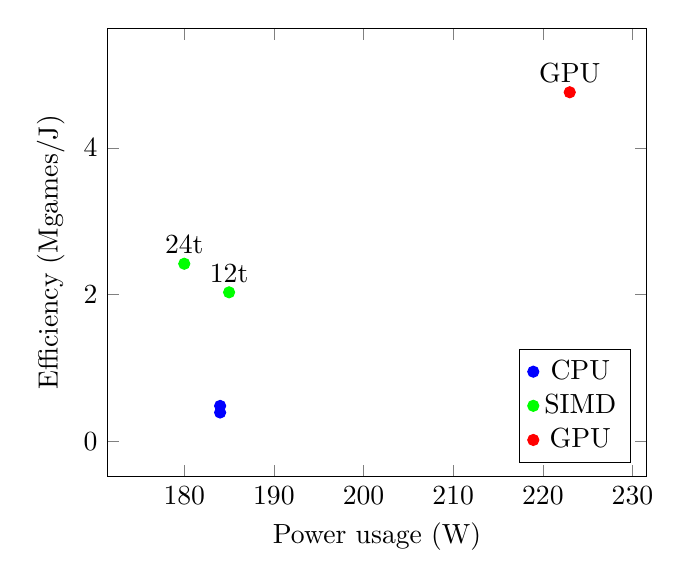
\begin{tikzpicture}
      \begin{axis}[enlargelimits=0.2, legend pos=south east, xlabel={Power usage (W)}, ylabel={Efficiency (Mgames/J)}]
        \addplot[
        scatter/classes={cpu={blue}, simd={green}, gpu={red}},
        scatter, mark=*, only marks, 
        scatter src=explicit symbolic,
        nodes near coords*={\Label},
        visualization depends on={value \thisrow{label} \as \Label}
        ] table [meta=class] {
          x y class label
          184 0.39 cpu {}
          184 0.48 cpu {}
          185 2.03 simd 12t
          180 2.42 simd 24t
          223 4.76 gpu GPU
        };
        \legend{CPU, SIMD, GPU};
      \end{axis}
    \end{tikzpicture}
  \end{center}
\end{frame}

\begin{frame}
  \frametitle{Enough optimising -- let's just get more hardware}

  \emph{RMIT AWS Cloud Supercomputing} (RACE) has kindly offered credit for
  using cloud computing for this project.

  They have newer GPUs: $5\times$ the FLOPS in from one Nvidia A10G GPU.
  
  They have more GPUs: a \emph{g5.48xlarge} computer has eight.
  1.6 days seems like a good guess\pause{} as I haven't benchmarked.
  I can't log into the portal.

  Budget may or may not be a problem; renting such a computer isn't cheap.
\end{frame}

\begin{frame}
  \frametitle{Unobscuring platypodes by clouds}

  \begin{center}
    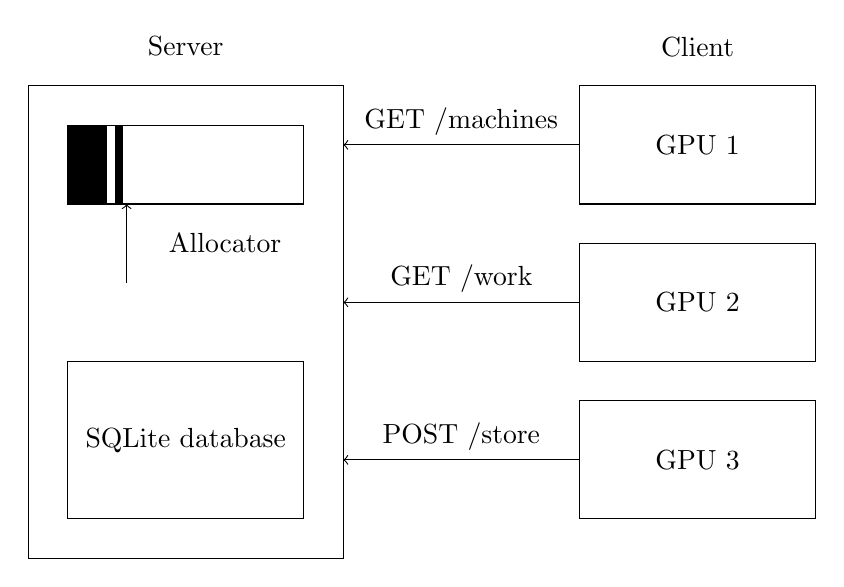
\begin{tikzpicture}
      % Server
      \node at (2, 6.5) {Server};
      \draw (0, 0) rectangle (4, 6);
      % - SQLite
      \draw (0.5, 0.5) rectangle (3.5, 2.5);
      \node at (2, 1.5) {SQLite database};
      % - Bitmap
      \draw (0.5, 4.5) rectangle (3.5, 5.5);
      \fill (0.5, 4.5) rectangle (1.0, 5.5);
      \fill (1.1, 4.5) rectangle (1.2, 5.5);
      \draw[->] (1.25, 3.5) -- (1.25, 4.5);
      \node at (2.5, 4) {Allocator};
      % - Client
      \node at (8.5, 6.5) {Client};
      
      \draw (7, 4.5) rectangle (10, 6);
      \draw[->] (7, 5.25) to node[midway, above] {GET /machines} (4, 5.25);
      \node at (8.5, 5.25) {GPU 1};
      
      \draw (7, 2.5) rectangle (10, 4);
      \draw[->] (7, 3.25) to node[midway, above] {GET /work} (4, 3.25);
      \node at (8.5, 3.25) {GPU 2};
      
      \draw (7, 0.5) rectangle (10, 2);
      \draw[->] (7, 1.25) to node[midway, above] {POST /store} (4, 1.25);
      \node at (8.5, 1.25) {GPU 3};
    \end{tikzpicture}
  \end{center}
\end{frame}

\end{document}

%%% Local Variables: 
%%% coding: utf-8
%%% mode: latex
%%% TeX-engine: xetex
%%% End: 